
% Frame ---------------------------------------------------------------------
\begin{frame}
\frametitle{Modelo de cámara}

\begin{block}{Definición - Cámara}
Una cámara es definida matemáticamente como una correspondencia entre el mundo 3D y una imagen 2D. Es decir, un mapeo entre puntos del mundo 3D $\point$ y puntos de la imagen $\imagePoint$:
\begin{equation}
\point=\begin{bmatrix}x\\
y\\
z
\end{bmatrix}\longmapsto
\imagePoint=\begin{bmatrix}u\\
v
\end{bmatrix}
\end{equation}
\end{block}

\end{frame}


% Frame ---------------------------------------------------------------------
\begin{frame}
\frametitle{Modelo de cámara pinhole}

\begin{block}{Cámara pinhole}
El punto de la imagen $\imagePoint=\begin{bmatrix}u & v\end{bmatrix}^{\top}$ es determinado como la intersección entre el \emph{plano de la imagen} y el rayo que une el punto del mundo 3D $\point=\begin{bmatrix}x & y & z\end{bmatrix}^{\top}$ con el \emph{centro focal} $\cameraCenter$ de la cámara.
\end{block}

\begin{figure}[!htb]
	\centering
	\subfloat[]{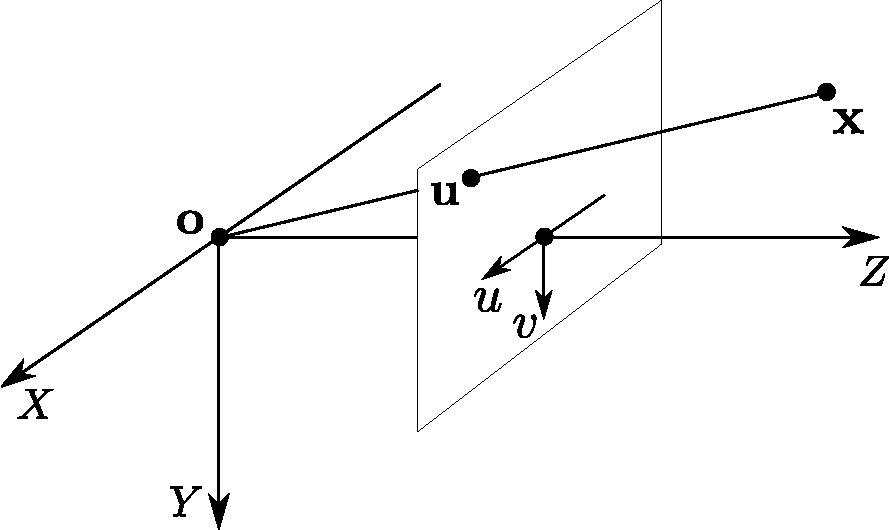
\includegraphics[width=0.5\columnwidth]{./cameras/pinhole_camera_model.pdf}}%
	\hfill
\end{figure}

\end{frame}


% Frame ---------------------------------------------------------------------
\begin{frame}
\frametitle{Modelo de cámara pinhole}

\begin{block}{Proyección central}
Asumiendo el centro focal en el origen de coordenadas y el plano de la imagen $Z=f$:

\begin{equation}
\begin{bmatrix}x\\
y\\
z
\end{bmatrix}\longmapsto\begin{bmatrix}fx/z\\
fy/z
\end{bmatrix}
\end{equation}

\end{block}

\begin{figure}[!htb]
	\centering
	\subfloat[]{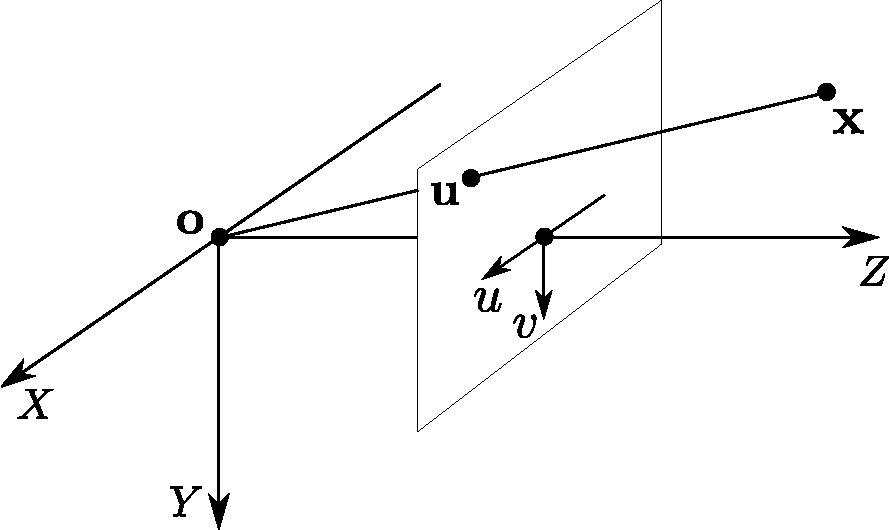
\includegraphics[width=0.5\columnwidth]{./cameras/pinhole_camera_model.pdf}}%
	\hfill
	\centering
	\subfloat[]{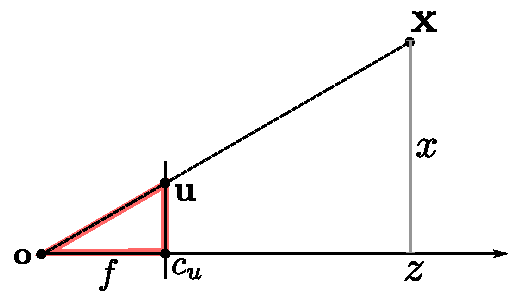
\includegraphics[width=0.5\columnwidth]{./cameras/pinhole_camera_model2.pdf}}%
	\hfill
\end{figure}

\end{frame}


% Frame ---------------------------------------------------------------------
\begin{frame}
\frametitle{Triangulación estéreo}

Proyecciones correspondientes $\imagePoint_{l}=\begin{bmatrix}u_{l} & v_{l}\end{bmatrix}$ y $\imagePoint_{r}=\begin{bmatrix}u_{r} & v_{r}\end{bmatrix}$ sobre los planos focales de la imagen izquierda y derecha respectivamente,
la posición del punto $\point$ puede ser derivada.

\begin{equation}
\frac{b}{z}=\frac{(b+u_{r})-u_{l}}{z-f}
\end{equation}

\begin{figure}[!htb]
	\centering
	\subfloat[]{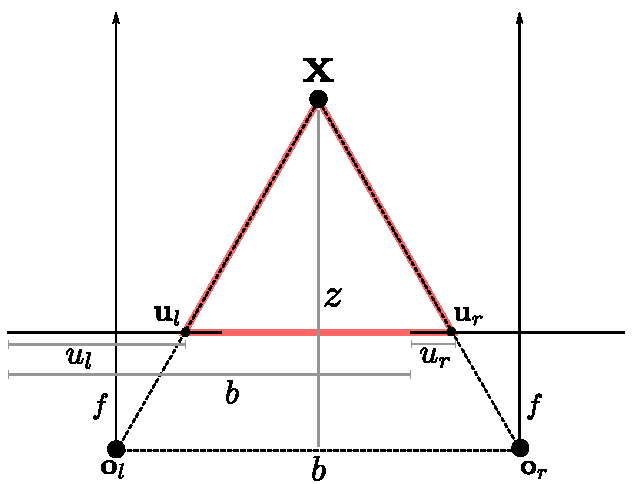
\includegraphics[width=0.5\columnwidth]{./cameras/stereo_triangulation.pdf}}%
	\hfill
	\centering
	\subfloat[]{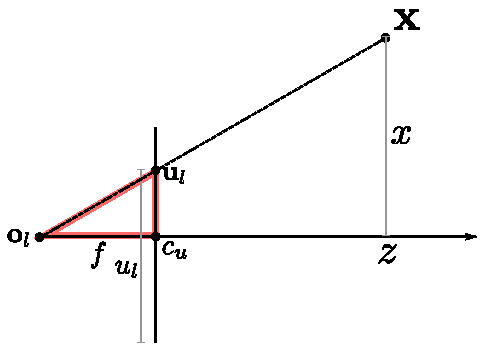
\includegraphics[width=0.5\columnwidth]{./cameras/stereo_triangulation2.pdf}}%
	\hfill
\end{figure}
\end{frame}


% Frame ---------------------------------------------------------------------
\begin{frame}
\frametitle{Triangulación estéreo}

\begin{equation}
\frac{x}{z}=\frac{u_{l}-c_{u}}{f}\qquad\frac{y}{z}=\frac{v_{l}-c_{v}}{f}
\end{equation}

\begin{equation}
\begin{aligned}x=\frac{(u_{l}-c_{u})z}{f}\;\qquad
y=\frac{(v_{l}-c_{v})z}{f}\;\qquad
z=\frac{bf}{u_{l}-u_{r}}\;
\end{aligned}
\end{equation}

\begin{figure}[!htb]
	\centering
	\subfloat[]{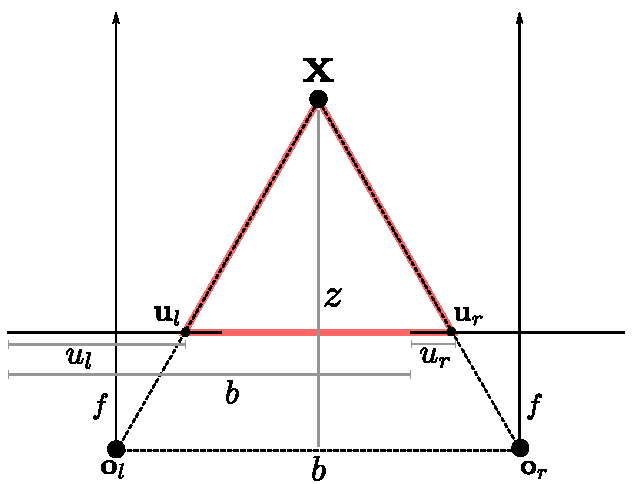
\includegraphics[width=0.5\columnwidth]{./cameras/stereo_triangulation.pdf}}%
	\hfill
	\centering
	\subfloat[]{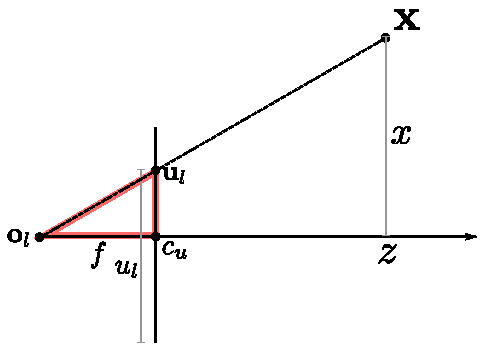
\includegraphics[width=0.5\columnwidth]{./cameras/stereo_triangulation2.pdf}}%
	\hfill
\end{figure}
\end{frame}


\subsection{Disparidad}


% Frame ---------------------------------------------------------------------
\begin{frame}
\frametitle{Disparidad}

\begin{block}{Definición - Disparidad}
La disparidad $d$ es definida como la distancia existente entre las proyecciones de las diferentes cámaras.
\begin{equation}
d=u_{l}-u_{r}=\frac{bf}{z}
\end{equation}
\end{block}

\textbf{Nota}: la profundidad $z$ es inversamente proporcional a la disparidad $d$.

\end{frame}

\begin{frame}
\frametitle{Modelo de cámara pinhole}

\pnote{* Lo anterior asume que el origen de coordenadas del plano de la imagen se encuentra en el punto principal. En la práctica, esto no siempre se cumple.}

\pnote{* Explicar representación en coordenadas homogéneas.}

Siendo $\begin{bmatrix}c_{u} & c_{v}\end{bmatrix}^{\top}$ la posición del punto principal.
\begin{equation}
\begin{bmatrix}x\\
y\\
z
\end{bmatrix}\longmapsto\begin{bmatrix}fx/z+c_{u}\\
fy/z+c_{v}
\end{bmatrix}
\end{equation}

En coordenadas homogéneas:

\begin{equation}
\begin{bmatrix}x\\
y\\
z\\
1
\end{bmatrix}\longmapsto\begin{bmatrix}fx+zc_{u}\\
fy+zc_{v}\\
z
\end{bmatrix}=\begin{bmatrix}f &  & c_{u} & 0\\
 & f & c_{v} & 0\\
 &  & 1 & 0
\end{bmatrix}\begin{bmatrix}x\\
y\\
z\\
1
\end{bmatrix}
\end{equation}

\begin{block}{Matriz de calibración intrínseca $\intrinsicMatrix$}
\begin{equation}
\intrinsicMatrix=\begin{bmatrix}f & 0 & c_{u}\\
0 & f & c_{v}\\
0 & 0 & 1
\end{bmatrix}
\end{equation}
\begin{equation}
\homo{\imagePoint}=\intrinsicMatrix\begin{bmatrix}\vec{{I}} & \vec{{0}}\end{bmatrix}\homo{\point}
\end{equation}
\end{block}

\end{frame}


\begin{frame}
\frametitle{Modelo de cámara pinhole}

\pnote{* Las ecuaciones anteriores deben extenderse agregando la transformación existente entre los sistemas de coordenadas de la cámara y el mundo.}

\pnote{* R es una matriz de rotación y t un vector de traslación.}

Puntos expresados en referencia al sistema de coordenadas del \textit{mundo}. La cámara no se encuentra necesariamente ubicada en el centro de este.

\begin{figure}[!htb]
	\centering
	\subfloat[]{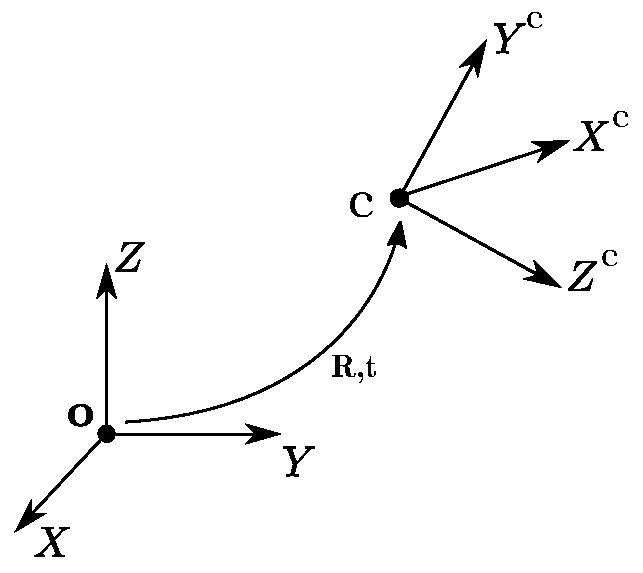
\includegraphics[width=0.4\columnwidth]{./cameras/camera_coord_system.pdf}}%
	\hfill
\end{figure}

\begin{block}{}
\begin{equation}
\homoCameraPoint=\begin{bmatrix}\rotation & \translation\\
0 & 1
\end{bmatrix}\begin{bmatrix}x\\
y\\
z\\
1
\end{bmatrix}=\seMatrix^{\mathrm{c}\mathrm{w}}\homoWorldPoint\;.
\end{equation}
\end{block}

\end{frame}


\begin{frame}
\frametitle{Modelo de cámara pinhole}

De esta manera, es posible proyectar cualquier punto 3D
$\homoWorldPoint$ en el sistema de coordenadas del mundo al correspondiente
punto $\homo{\imagePoint}$ en el plano de la imagen mediante:

\begin{block}{Matriz de proyección \textmd{$\projectionMatrix$}}
\begin{equation}
\projectionMatrix=\intrinsicMatrix\begin{bmatrix}\rotation & \translation\end{bmatrix}
\end{equation}
\begin{equation}
\homo{\imagePoint}=\projectionMatrix\homoWorldPoint
\end{equation}
\end{block}

\end{frame}


\begin{frame}
\frametitle{Modelo de cámara estéreo}

\begin{block}{Geometría epipolar}

\pnote{* La geometría proyectiva intrínseca entre dos cámaras es conocida como geometría epipolar.}

\pnote{* Esta es independiente de la escena observada y depende únicamente de los parámetros internos geometría epipolar y las posiciones relativas de las cámaras involucradas.}

Cualquier punto 3D $\point$ en el espacio, sus proyecciones $\imagePoint$ y $\imagePoint^{\prime}$ en los planos de las imágenes y los centros focales de las cámaras, pertenecen a un mismo plano $\vec{\pi}$.
De manera análoga, los rayos re-proyectados desde $\imagePoint$ y $\imagePoint^{\prime}$ se intersectan en $\point$, son coplanares y yacen sobre $\vec{\pi}$.
\end{block}

\begin{figure}[!htb]
	\centering
	\subfloat[]{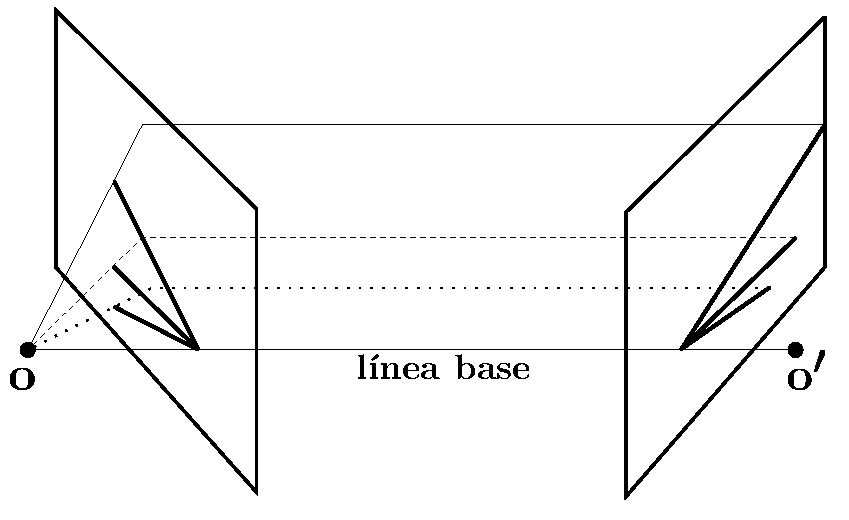
\includegraphics[width=0.5\columnwidth]{./cameras/pencil_of_planes.pdf}}%
	\hfill
	\centering
	\subfloat[]{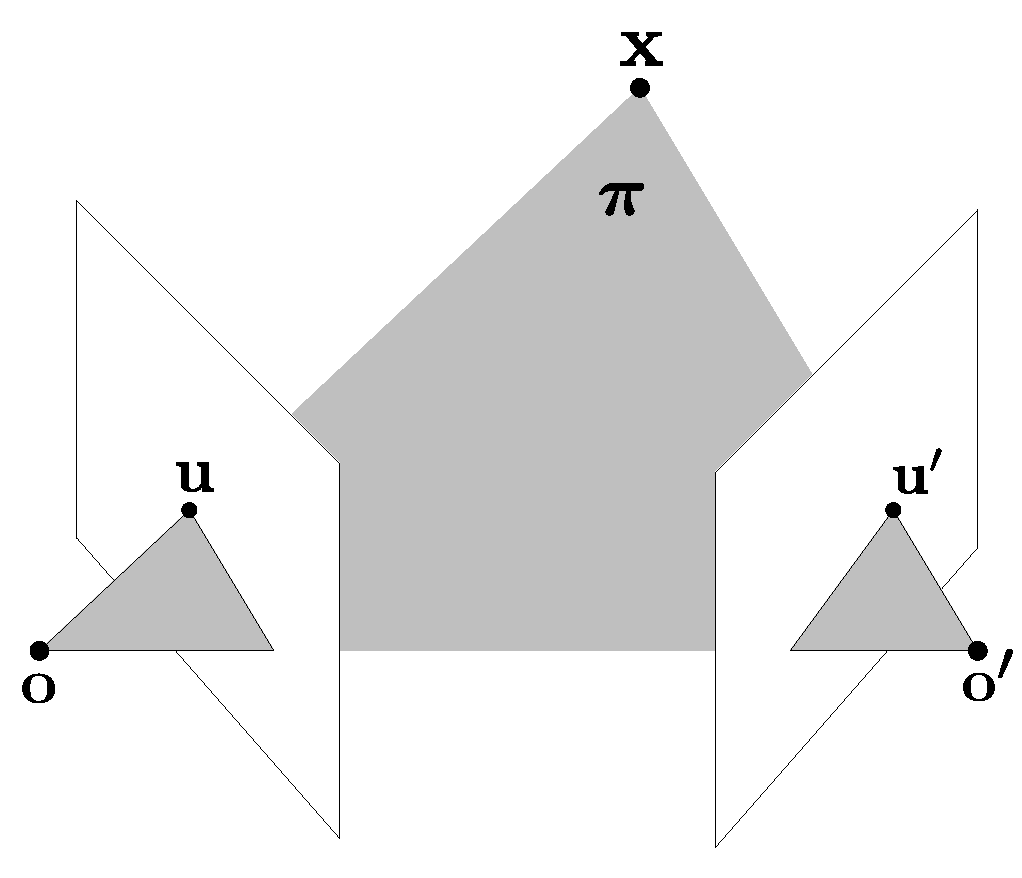
\includegraphics[width=0.5\columnwidth]{./cameras/epipolar_plane.pdf}}%
	\hfill
\end{figure}
\end{frame}


\begin{frame}
\frametitle{Modelo de cámara estéreo}

\pnote{* La búsqueda del correspondiente al punto u no necesita cubrir el plano de la imagen completo sino que puede restringirse a la línea epipolar l.}

\pnote{* La línea epipolar es generada por la proyección del rayo, re-proyectado desde u, sobre el plano focal de la segunda imagen.}

Búsqueda de correspondencias sobre la línea epipolar.

\begin{figure}[!htb]
	\centering
	\subfloat[]{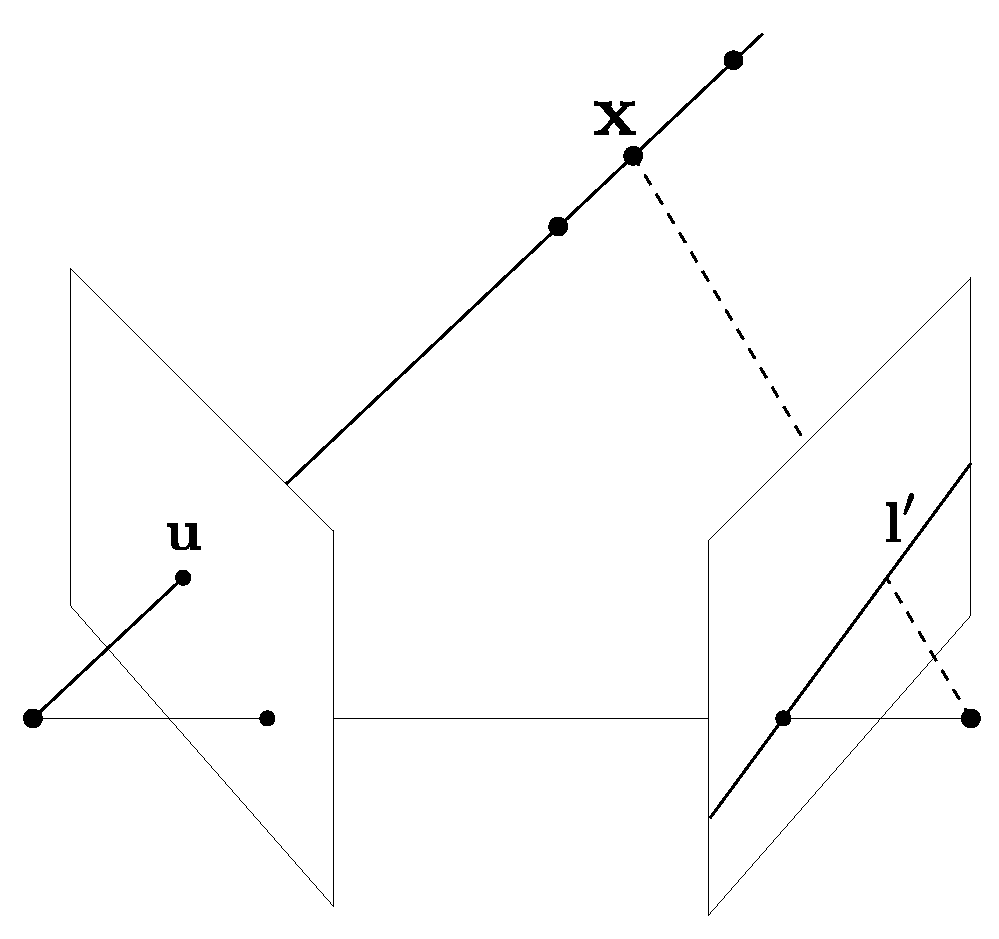
\includegraphics[width=0.5\columnwidth]{./cameras/epipolar_line.pdf}}%
	\hfill
\end{figure}
\end{frame}


\begin{frame}
\frametitle{Rectificación estéreo}

\pnote{* Luego de aplicar rectificación estéreo, la búsqueda de correspondencias entre las imágenes es reducida a una búsqueda unidimensional, sobre la misma fila.}

\begin{itemize}
\item Proyectar el par de imágenes estéreo sobre un plano de imagen común.
\item Los puntos correspondientes se encuentren alineados en la misma fila.
\end{itemize}

\begin{figure}[!htb]
	\centering
	\subfloat[]{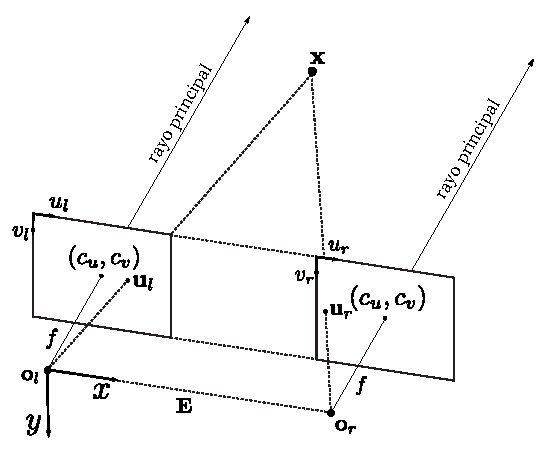
\includegraphics[width=0.6\columnwidth]{./cameras/stereo_rectification.pdf}}%
	\hfill
\end{figure}
\end{frame}


\begin{frame}
\frametitle{Rectificación estéreo}

\pnote{* Rectificación estéreo sobre un par de imágenes del Dataset Level 7 [32]. (a) Par de imágenes estéreo original provisto por la cámara estéreo.}
\pnote{* (b) El par de imágenes estéreo luego de ser rectificadas. Las líneas rojas asocian algunos puntos correspondientes entre ambas imágenes. Notar que estos puntos se encuentran en la misma fila en ambas imágenes.}

\begin{figure}[!htb]
	\centering
	\subfloat[]{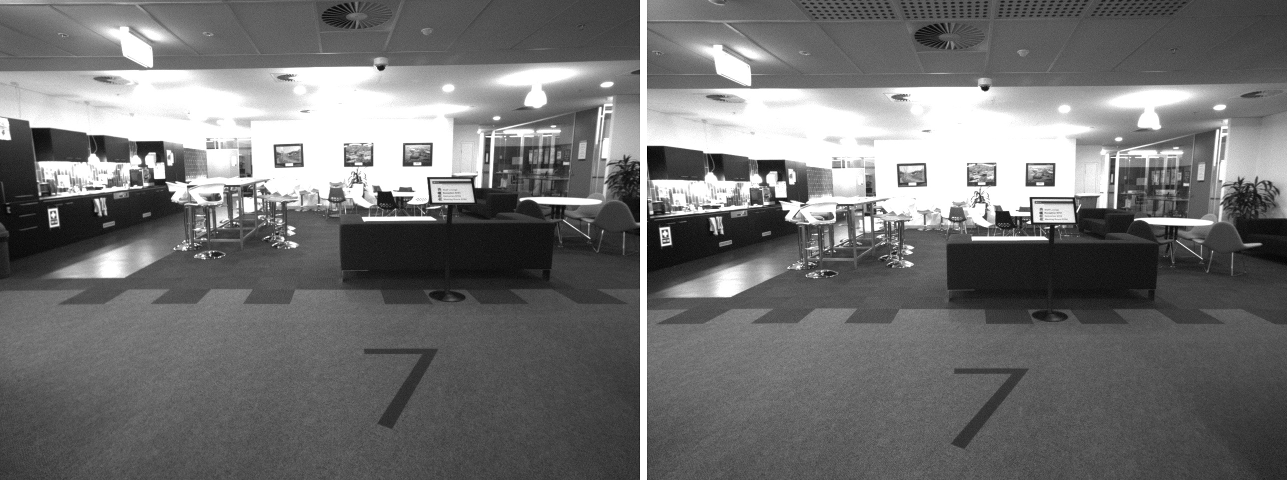
\includegraphics[width=0.6\columnwidth]{./cameras/no_rectified_stereo_images.png}}%
	\hfill
	\\
	\centering
	\subfloat[]{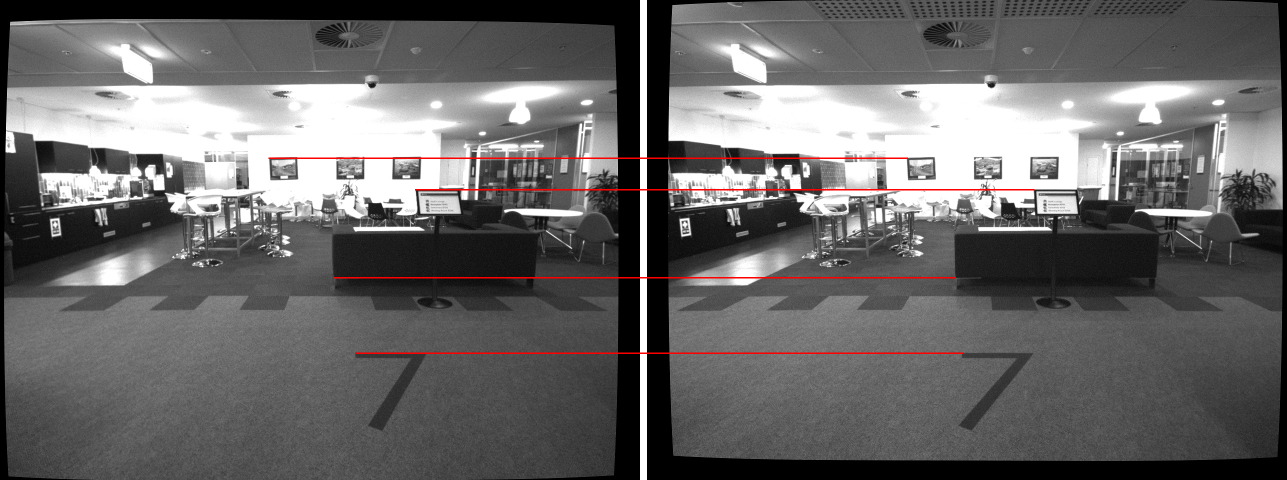
\includegraphics[width=0.6\columnwidth]{./cameras/rectified_stereo_images.png}}%
	\hfill
\end{figure}
\end{frame}


\begin{frame}
	\frametitle{S-PTAM}
	\begin{figure}[htb]
		\centering
		
\includegraphics[width=1.0\columnwidth]{method/portada-sptam-kitti-video.pdf}
		\hfill
	\end{figure}

\end{frame}

% Frame ---------------------------------------------------------------------
\begin{frame}
	\frametitle{Expansión y fusión de mapa: Frustrum culling}
	\begin{itemize}
		\item Empleando la posición del keyframe $\keyframe_{j}$ se proyecta el \emph{mapa local}: últimas $J$ \emph{nubes de puntos} $\left\{ \pointCloud_{j-J},\hdots,\pointCloud_{j-1}\right\}$.
		\begin{itemize}
			\item Aplicando \emph{Frustum culling} para filtrar puntos no-visibles.
		\end{itemize}
	\item Utilizando el mapa de disparidad del \emph{keyframe} actual $\keyframe_{j}$ se buscan correspondencias.
	\end{itemize}
	
	\begin{figure}[htb]
		\centering
		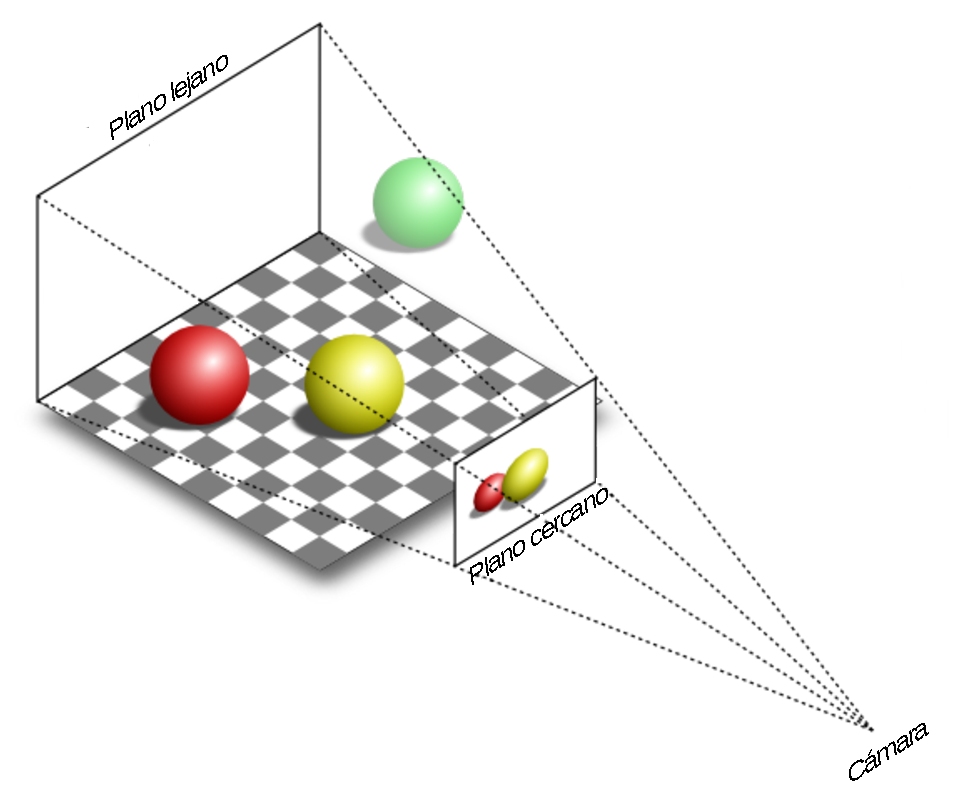
\includegraphics[width=0.6\columnwidth]{method/frustum_culling.pdf}
	\end{figure}

\end{frame}

% Frame ---------------------------------------------------------------------
\begin{frame}
	\frametitle{ROS: Robot Operating System}
    \begin{figure}[htb]
        \centering
        
\includegraphics[width=0.55\columnwidth]{method/ros.png}
    \end{figure}
	\vspace{-2em}
    \begin{itemize}
 		\item Conjunto de frameworks para desarrollo de software en robótica.
        \item Abstracción del hardware.
        \item Control de dispositivos de bajo nivel.
        \item Arquitectura:
            \begin{itemize}
	        	\item Cada nodo es una unidad de ejecución.
	        	\item Comunicación entre nodos mediante mensajes.
	        \end{itemize}
        \item Mantenimiento de paquetes.
        \item Utilizado en la comunidad robótica.
    \end{itemize}
\end{frame}


% Frame ---------------------------------------------------------------------
\begin{frame}
	\frametitle{ROS: Robot Operating System}
	
	\begin{figure}[htb]
		\subfloat[] {
			\begin{tabular}[b]{c}
				\centering
				$\vcenter{\hbox{
\includegraphics[width=0.15\columnwidth]{./method/opencv.png}}}$
				\hspace{1em}
				$\vcenter{\hbox{
\includegraphics[width=0.25\columnwidth]{./method/ros.png}}}$
				\hspace{1em}
				$\vcenter{\hbox{
\includegraphics[width=0.25\columnwidth]{./method/pcl.png}}}$
			\end{tabular}
		}
	\end{figure}
	
	\vspace{-2em}
	\begin{itemize}
		\item Implementado como un nodo ROS.
		\item Código fuente disponible públicamente bajo licencia (GPLv3) \url{https://github.com/CIFASIS/dense-sptam}.
		\item Librerías:
		\begin{itemize}
			\item OpenCV: manejo y codificación de imágenes.
			\item Point Cloud Library (PCL): manejo de nubes de puntos.
			\item LIBELAS: cómputo de mapas de disparidad.
		\end{itemize}
		\item Compuesto de 3 hilos de ejecución paralela.
    \end{itemize}
\end{frame}


% Frame ---------------------------------------------------------------------
\begin{frame}
	\frametitle{KITTI: error de mediana}
	\centering
	Comparación de mediana de error (profundidad vs. error).
	\vspace{-1em}
	\begin{figure}[!htb]
		\captionsetup{justification=centering}
		\subfloat[KITTI 00]{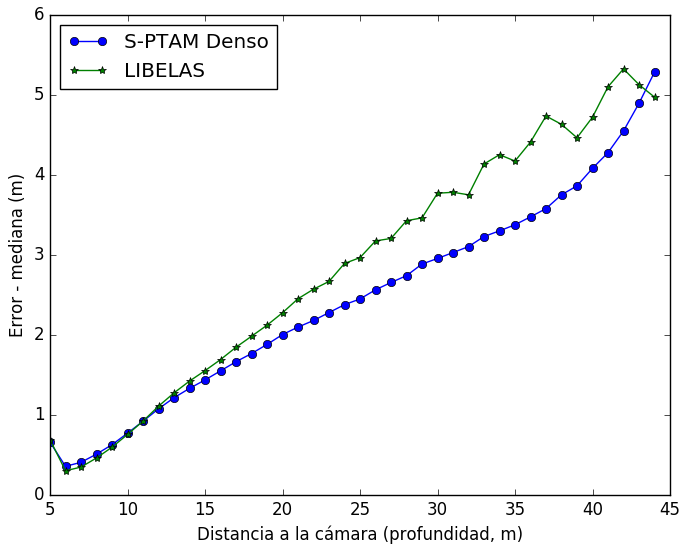
\includegraphics[width=0.35\columnwidth]{./experiments/kitti_medians/00.png}%
		}
		\hfil
		\subfloat[KITTI 01]{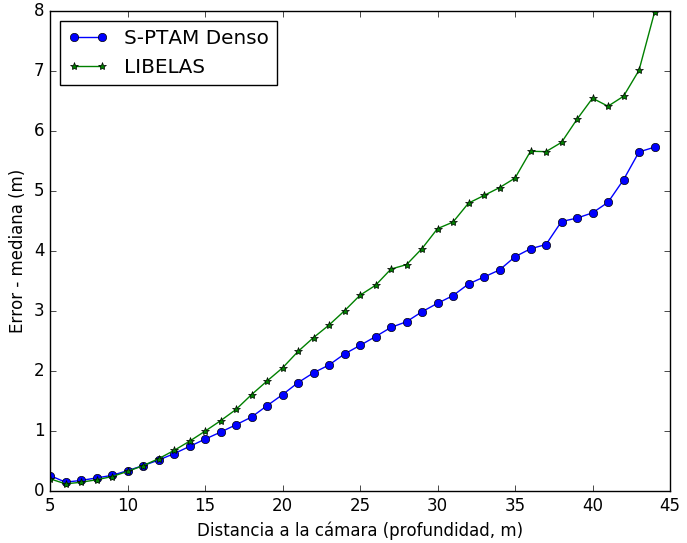
\includegraphics[width=0.35\columnwidth]{./experiments/kitti_medians/01.png}%
		}
	\end{figure}
	\vspace{-2em}
	\begin{figure}[!htb]
		\captionsetup{justification=centering}
		\subfloat[KITTI 02]{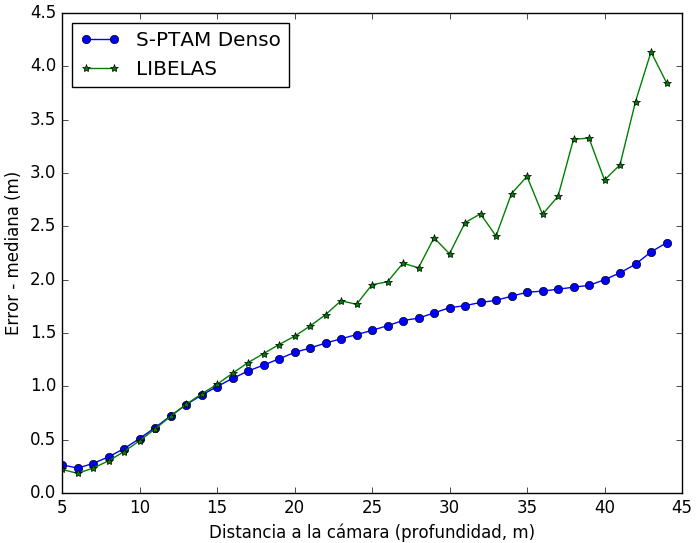
\includegraphics[width=0.35\columnwidth]{./experiments/kitti_medians/02.png}%
		}
		\hfil
		\subfloat[KITTI 03]{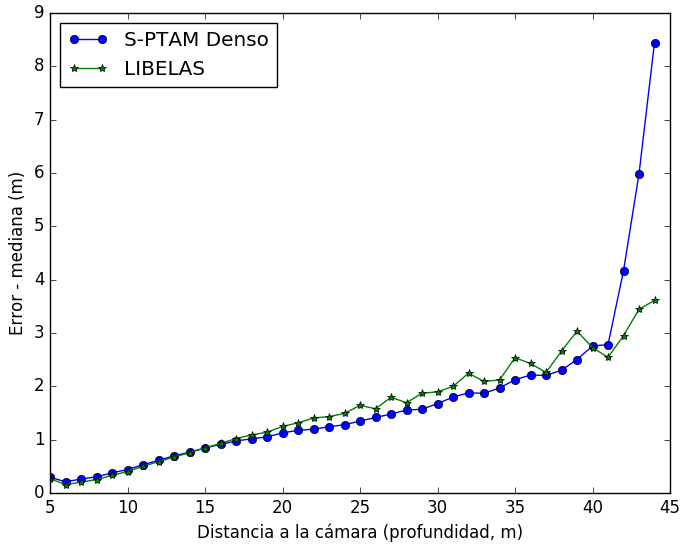
\includegraphics[width=0.35\columnwidth]{./experiments/kitti_medians/03.png}%
		}
	\end{figure}
\end{frame}


% Frame ---------------------------------------------------------------------
\begin{frame}
	\frametitle{KITTI: error de mediana}
	\centering
	Comparación de mediana de error (profundidad vs. error).
	\vspace{-1em}
	\begin{figure}[!htb]
		\captionsetup{justification=centering}
		\subfloat[KITTI 04]{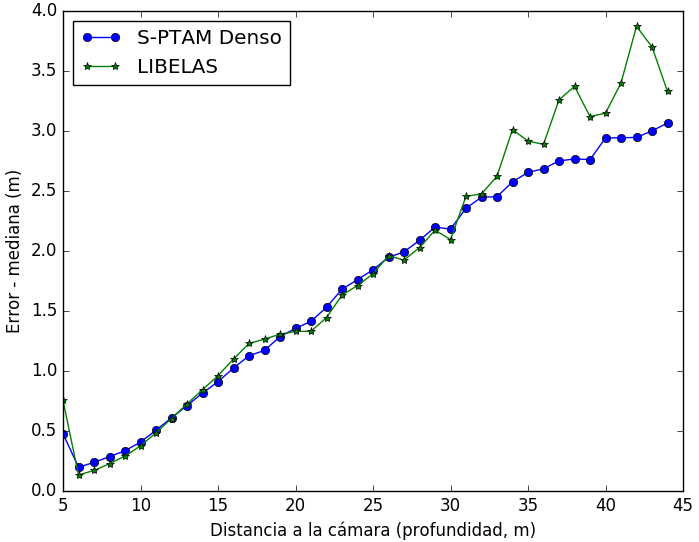
\includegraphics[width=0.35\columnwidth]{./experiments/kitti_medians/04.png}%
		}
		\hfil
		\subfloat[KITTI 05]{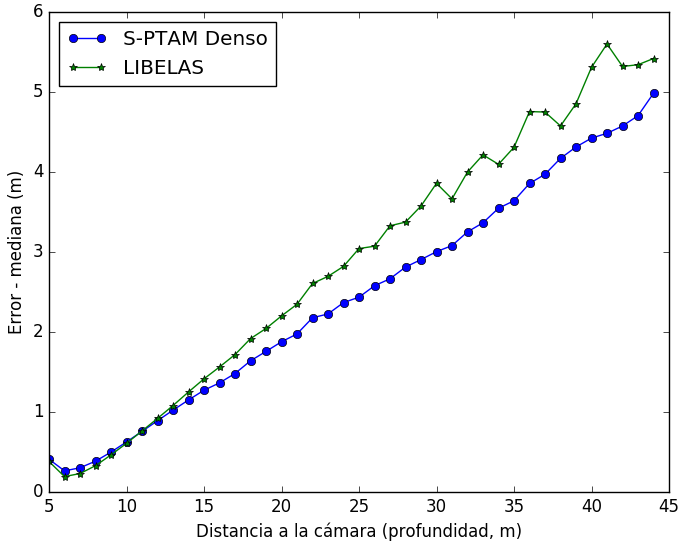
\includegraphics[width=0.35\columnwidth]{./experiments/kitti_medians/05.png}%
		}
	\end{figure}
	\vspace{-2em}
	\begin{figure}[!htb]
		\captionsetup{justification=centering}
		\subfloat[KITTI 07]{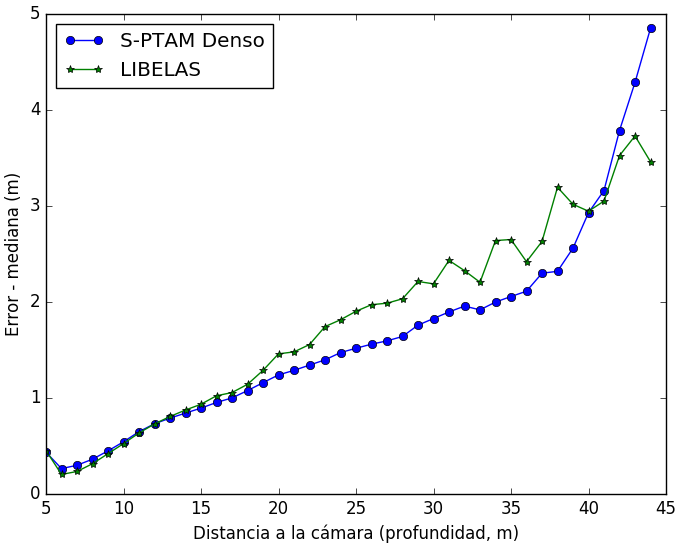
\includegraphics[width=0.35\columnwidth]{./experiments/kitti_medians/07.png}%
		}
		\hfil
		\subfloat[KITTI 08]{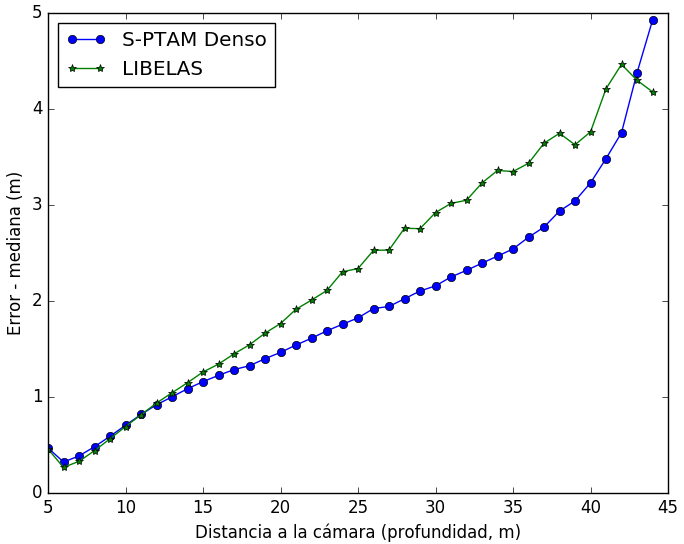
\includegraphics[width=0.35\columnwidth]{./experiments/kitti_medians/08.png}%
		}
	\end{figure}
\end{frame}


% Frame ---------------------------------------------------------------------
\begin{frame}
	\frametitle{KITTI: error de mediana}
	\centering
	Comparación de mediana de error (profundidad vs. error).
	\vspace{-1em}
	\begin{figure}[!htb]
		\captionsetup{justification=centering}
		\subfloat[KITTI 09]{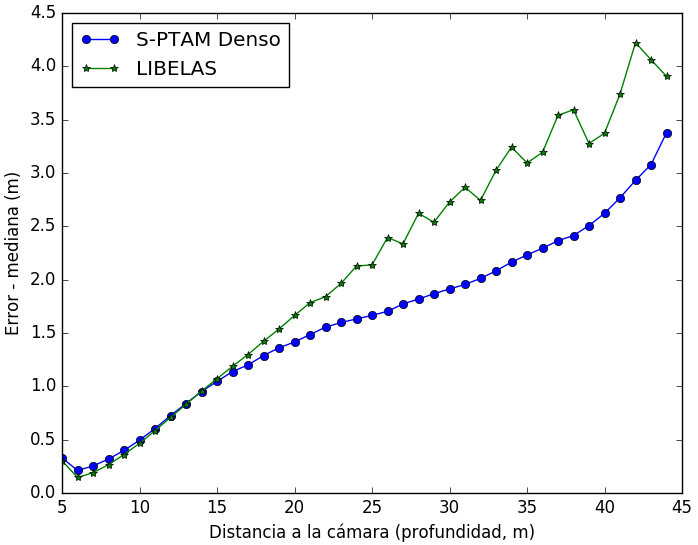
\includegraphics[width=0.35\columnwidth]{./experiments/kitti_medians/09.png}%
		}
		\hfil
		\subfloat[KITTI 10]{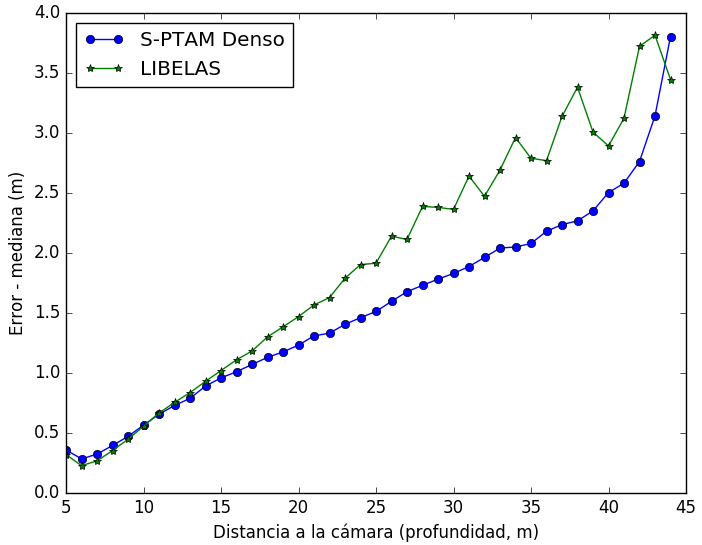
\includegraphics[width=0.35\columnwidth]{./experiments/kitti_medians/10.png}%
		}
	\end{figure}
\end{frame}


% Frame ---------------------------------------------------------------------
\begin{frame}
	\frametitle{Análisis de tiempos}
	\vspace{-0.7em}
	\begin{center}
	\begin{figure}[tbh]
	\begin{centering}
	\begin{tabular}{cccc}
		\toprule 
		Secuencia & Disparidad & Expansión y fusión & Refinamiento\tabularnewline
		\midrule
		\midrule 
		Tsukuba & 118.20 & 132.72 & 4.80\tabularnewline
		\midrule 
		KITTI 00 & 156.92 & 115.40 & 6.53\tabularnewline
		\midrule 
		KITTI 01 & 156.10 & 69.12 & 5.21\tabularnewline
		\midrule 
		KITTI 02 & 160.63 & 108.13 & 6.58\tabularnewline
		\midrule 
		KITTI 03 & 153.66 & 83.01 & 4.83\tabularnewline
		\midrule 
		KITTI 04 & 149.15 & 72.99 & 5.00\tabularnewline
		\midrule 
		KITTI 05 & 165.31 & 108.97 & 5.97\tabularnewline
		\midrule 
		KITTI 06 & 154.89 & 83.21 & 4.84\tabularnewline
		\midrule 
		KITTI 07 & 155.74 & 113.15 & 6.10\tabularnewline
		\midrule 
		KITTI 08 & 152.10 & 101.01 & 5.22\tabularnewline
		\midrule 
		KITTI 09 & 159.84 & 101.20 & 5.76\tabularnewline
		\midrule 
		KITTI 10 & 158.81 & 117.42 & 6.35\tabularnewline
		\bottomrule
	\end{tabular}
	\par\end{centering}
	\centering
	\caption{Tiempo de computación promedio (en ms) para cada fase.}
	\end{figure}
	\par\end{center}
\end{frame}

